\documentclass[a4,12pt]{scrartcl}

%Basic 
\usepackage[utf8]{inputenc}
\usepackage[ngerman]{babel}
\usepackage[T1]{fontenc}
\usepackage{float}
\usepackage[bottom = 3.50cm]{geometry}

%Titel Seite
\title{CLOUD INFRASTRUCTURE}
\subtitle{Lab-04}
\author{Giorgio Vincenti und Samuel Krieg}
\date{\today}


%Kopf, Fusszeile
\usepackage{fancyhdr}
\pagestyle{fancy}
\lhead{ \begin{picture}(0,0) \put(0,0){
\includegraphics[width=3cm]{./pictures/hsrlogo.png}} \end{picture}}
\chead{}
\rhead{Seite \thepage}
\lfoot{Cloud Infrastructure \\Lab-04}
\cfoot{Giorgio Vincenti und Samuel Krieg}
\rfoot{\today}
\renewcommand{\headrulewidth}{0.4pt}

%Bilder
\usepackage{graphicx}
\usepackage{wrapfig}


%Tabellen
\usepackage{booktabs}

%Querformat für eine Seite
\usepackage{lscape}
\usepackage{rotating}
\usepackage{pdflscape}

%Temp
\usepackage{lipsum}



\begin{document}

\clearpage\maketitle
\thispagestyle{empty}
\tableofcontents
\newpage

\section{Aufgabenstellung}
Wurde aus der Aufgabenstellung entnommen: \newline
\newline
Your teammate needs your help. She works in the software development team and is not really experienced in Linux server and virtualization. Create a How-to for your workmate in order that the software developer can use it.
\newline
\newline
What they need:
\begin{itemize}
\item 3 separated virtual machines
\item  VM1 has to be reachable from the internet and needs connectivity to VM2
\item VM2 needs connectivity to VM3
\item It has to be runnable on a virtual Linux server without GUI
\item Guess how long it will take for the SE
\end{itemize}

Add the following to your delivery:
\begin{itemize}
\item Usability
\item Is it possible to deploy the VMs on multiple hosts (2 Nodes)?
\end{itemize}

Hints
\begin{itemize}
\item Download Qcow image for VM
\item Qemu supports different network backend types
\item Guest VM don’t need a GUI
\end{itemize}

\subsection{Wichtiges im Überblick}
Hier einen Überblick über die erforderlichen Punkte:
\begin{itemize}
\item Anleitung für Software Engineering 
\begin{itemize}
\item Anleitung für erstellen / verwalten von VMs
\end{itemize}
\item 3 virtuelle Maschinen installieren
\item VM1 muss vom Internet aus erreichbar sein
\item VM2 muss mit VM3 kommunizieren können
\item Dauer einer Installation abschätzen / messen
\item Verwendbarkeit aufzeigen
\item Einsatz der VMs auf mehreren Hosts abklären
\end{itemize}

\subsection{Kriterien}
Wurden aus dem Mail von Urs Baumann entnommen: 
\begin{itemize}
\item Struktur
\item Verständlich für Software Entwickler
\item Funktionalität 
\item Kapitel zu Usability 
\item Eingesetzte Netzwerktypen 
\item Kapitel zu "multi host setup"  
\end{itemize}
\newpage

\section{Infrastruktur}
Hier einige Eckdaten zu der Infrastruktur. 

\subsection{Virtualisierungs-Software}
Als Virtualisierungssoftware wird VMWare Workstation eingesetzt. 

\subsection{Virtualisierungs-Host}
Als Virtualisierungs-Host wir ein Linux Server OS eingsetzt. Wir gehen nicht auf die Details der Installation ein. Es wird nur das nötigste dokumentiert.  

\subsubsection{OS} 
Hier einige Details über die eingesetzte Linux Distribution. 
\begin{center}
    \begin{tabular}{@{} l l r@{}}\toprule    
    {Linux Distribution} & {Version}\\ \midrule
    Ubuntu & Server x.x.x.x\\ \addlinespace
    \bottomrule
    \end{tabular}
\end{center}

\subsubsection{Login}
Es sind zwei Logins auf dem Server eingerichtet. Eines für die Userin, um VMs erstellen zu können und eines für die Administratoren um den Server zu verwalten. 
\begin{center}
    \begin{tabular}{@{} l l r@{}}\toprule    
    {Benutzername} & {Passwort} & {Privilegien}\\ \midrule
    HSR & hsr & User\\ \addlinespace
    root & ****** & Administrator\\ \addlinespace
    \bottomrule
    \end{tabular}
\end{center}

\subsubsection{Network}
Der Server verfügt über eine statische IP-Konfiguration. Über diese IP kann der Server verwaltet werden. 
\begin{center}
    \begin{tabular}{@{} l l r@{}}\toprule    
    {Hostname} & {IP-Adresse} & {Subnetz}\\ \midrule
    SE01 & 10.0.1.11 & 255.255.255.0\\ \addlinespace
    \bottomrule
    \end{tabular}
\end{center}

\subsubsection{Services}
Auf dem Server laufen keine, für die Umgebung relevanten, Services. 

\subsubsection{Application}

\newpage
\subsubsection{Verwaltung}
Um den Server von Remote zu verwalten empfehlen wir SSH Secure Shell oder PuTTy. Diese Tools kann man kostenlos vom Internet heruntergeladen und verwenden. Der Server kann auch per Konsole verwaltet werden.
\begin{figure} [H]
\begin{center}
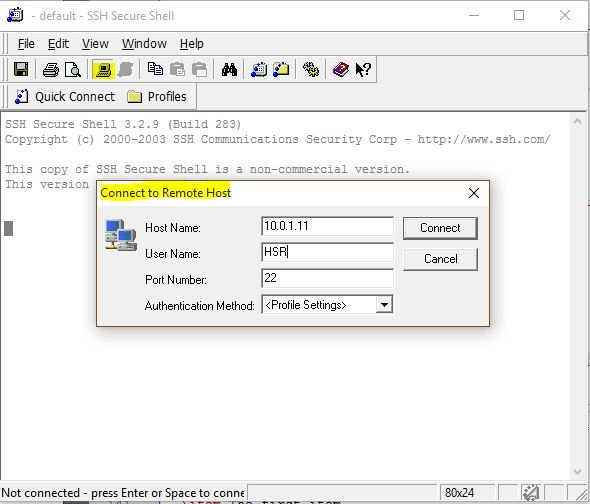
\includegraphics[width=0.48\textwidth]{./pictures/ssh_login.jpg}
\caption{Login in SSH Secure Shell}
\end{center}
\end{figure}

\subsection{Virtualisierungs-Guests}
Die Umgebung besteht aus gesamt drei virtuellen Guests, die auf dem Virtualisierungs-Host laufen. 
\subsubsection{VM1 - bla bla}
\subsubsection{VM2 - bla bla}
\subsubsection{VM3 - bla bla}
\newpage
\subsection{Enumerate}
\begin{enumerate}
  \item The first item
  \item The second item
  \item The third etc \ldots
\end{enumerate}

\subsubsection{Subsubsection}
Text

\subsection{Description}
\begin{description}
  \item[First] The first item
  \item[Second] The second item
  \item[Third] The third etc \ldots
\end{description}

\section{Anleitung}
\newpage

\end{document}
